\section{Class 4 - 5/03/21}
\subsection*{Transmission line}
When we have a signal to be transmitted over a cable, the problem to connect the source of the signal to the load is not as simple as cabling a dc power source. In our case the voltage level to be transmitted can be considered as a wave, and his behavior over the transmission line can vary with the length, the frequency of the signal or also with the geometry of the cable.
\begin{figure}[H]
\begin{center}
    \begin{circuitikz} [ baseline=(current bounding box.center)]
        \ctikzset { label/align = straight }
        \node[draw,minimum width=4cm,minimum height=2.4cm,anchor=south west] at (2.5,-0.2){TL};
        \draw (0,0)
        to[sV=$V_{g}$] (0,2)
        to[R=$R_{g}$, -o] (2,2)
        node[label={[font=\footnotesize]above:$A$}] {}
        to[short] (2.5,2)
        (0,0) to[short, -o] (2,0) 
        node[label={[font=\footnotesize]below:$A'$}] {}
        to[short] (2.5,0);
        \draw (8.5,0) 
        to[short, -o] (7.,0)
        node[label={[font=\footnotesize]below:$B'$}] {}
        to[short](6.5,0)
        (8.5,2) to[generic=$Z_{l}$] (8.5,0)
        (8.5,2) to[short, -o] (7,2)
        node[label={[font=\footnotesize]above:$B$}] {}
        to[short](6.5,2)
        ;
      \end{circuitikz}     
\end{center} \caption{Transmission line example} \label{fig:transmission_line_example}
\end{figure}
In \cref{fig:transmission_line_example} a very simplified view of a transmission line, where the voltage at the input is the one over $AA'$, and $BB'$ on the output.\\
If we do not consider the resistance $R_g$, then the voltage in input of the TL can be seen as:
\begin{equation}
  V_{AA'}(t)=V_g(t)=V_0 \, \cos(\omega t)
\end{equation}
Now for the output voltage equation we need to consider the time delay of signal travelling from $A$ to $B$. So we need to consider the same signal $V_{AA'}$ but delayed by $\frac{l}{c}$ ($l$ is the length of the TL, and $c$ is the speed of the signal, the same speed of light).
\begin{align}\label{eq:vbb_in_transmission_line}
  \begin{split}
    V_{BB'}(t)&=V_{AA'}\left(t-\frac{l}{c}\right)=\\[5pt]
      &=V_0 \, \cos\left[\omega \left(t-\frac{l}{c}\right)\right]=\\[5pt]
      &=V_0\, \cos\left(\omega t-\frac{\omega}{c}\, l\right)=\\[5pt]
      &=V_0\, \cos\left(\omega t-\beta\, l\right)= \\[5pt]
  \end{split}
\end{align}
Actually in \cref{eq:vbb_in_transmission_line} we can see that our signal over the transmission line is actually a wave dependent on the frequency and the length of the cables.
\subsection*{Example on different transmission line length}
As we can see in \cref{eq:vbb_in_transmission_line}, we need to face a new problem: how the strength of our signal change accordingly to the length of my transmission line?\\
For example, on the input of the TL we have a signal with amplitude $A_0$ and a frequency of $f=\SI{1}{\kilo\hertz}$.\\
Suppose the length of the TL $l=\SI{5}{\centi \meter}$, then the signal on the output at $t=0$ will be:
\begin{align*}
  \begin{split}
  V_{BB'}(t)&=V_0\, \cos\left(\omega t-\beta\, l\right)=\cos\left(\omega t-\frac{\omega}{c}\, l\right)=\\[5pt]
  &=V_0\, \cos\left(2\,\pi\,10^{3}\cdot 0+\frac{2\,\pi\,10^{3}}{3\cdot 10^{8}}\cdot 0.05\right)=\\[5pt]
  &=V_0\,\cos(0,105 \cdot 10^{-5})\approx V_0\cdot 0.999\approx V_0
  \end{split}
\end{align*}
As we can see, we have a very short length of the cable compared to the wavelength, the attenuation over the line due is totally negligible.\\
If we suppose instead the length of the TL: $l=\SI{100}{\kilo \meter}$, then the signal on the output at $t=0$ will be:
\begin{align*}
  \begin{split}
  V_{BB'}(t)&=V_0\, \cos\left(2\,\pi\,10^{3}\cdot 0+\frac{2\,\pi\,10^{3}}{3\cdot 10^{8}}\cdot100\cdot 10^{3}\right)=\\[5pt]
  &=V_0\,\cos(2.09)\approx V_0\cdot -0.49\approx -\frac{1}{2}\,V_0
  \end{split}
\end{align*}
It is very important to notice that now the amplitude of the signal is half as before, just by moving away from the source, and without considering the attenuation of the line.\\
This behavior can be explained by looking at the argument of the $cos$ on \cref{eq:vbb_in_transmission_line}: 
\begin{itemize}
  \item $\bm{(\omega t)}$ : is responsible to the information propagation (otherwise we could not detect the wave).
  \item $\bm{(\beta\, l)}$ : is the one dependent on the length that we need to investigate.
\end{itemize}
What we can notice is that the effect of that attenuation depends a lot on the wavelength:
\begin{equation*}
  \beta\, l=\frac{\omega}{c}\,l=\frac{2\pi}{c}\cdot f\cdot l=2\pi\cdot\frac{l}{\lambda}
\end{equation*}
The cosine operator is periodic over $2\pi$, this mean that when the length of the TL $l$ is a multiple of the wavelength $\lambda$, the output signal won't be attenuated: $\cos(k\,2\pi)=1$.\\
But when $l = (\frac{n}{2}+1)\,\lambda$ for $n=0,1,\cdots$ at $t=0$, on the output of the TL we will not see any signal because $\cos(k\,\frac{\pi}{2})=1$\\
Now you could say: \textit{"hey!, that sounds like a simple phase shift, we can just wait $\frac{\pi}{2}$ and then the signal amplitude will be again $A_0$"}, that is true my friend, but by this example it is very simple to understand how a signal can change if we move over a transmission line.\\
In the next section we will talk about a real attenuation of the signal along the TL (for example we will be able to choose the right distance from the source to guarantee the maximum power transfer).\\
Another thing that we will take in consideration is the losses over the line, and the attenuation of the reflected signal.
\subsubsection*{How can we model our transmission line?}
To propagate an electric signal we need 2 conductors, it is not important if they are twisted pairs or coaxial (for now).\\
Then we can divide our line in different sectors of length $\Delta z$, and each segment can be modelled as a circuit:
\begin{figure}[H]
  \begin{center}
      \begin{circuitikz} [ baseline=(current bounding box.center)]
          \ctikzset { label/align = straight }
          \draw (8,0)
          to[short, o-o,] (0,0)
          (0,4)
          to[R=$R\,\Delta z$,o-] (2,4)
          to[L=$L\,\Delta z$] (4,4)
          to[short,-o](8,4)
          (4,4)to[short](4,3)
          (3,3)to[short](5,3)
          (3,1)to[short](5,1)
          (4,0)to[short](4,1)
          (5,3)to[C=$C\,\Delta z$](5,1)
          (3,1)to[R=$G\,\Delta z$](3,3)
          ;
          \draw [decorate,decoration={brace,amplitude=6pt,mirror,raise=1ex}]
          (0,0) -- (8,0) node[midway,yshift=-2em]{$\Delta z$};
        \end{circuitikz}     
  \end{center} \caption{Circuital representation of a TL section} \label{fig:transmission_section_delta_z}
\end{figure}
Now from \cref{fig:transmission_section_delta_z} we can see different parameters:
\begin{itemize}
  \item $\bm{R\,\Delta z}$ : Resistance representing the losses on both conductors along the line.
  \item $\bm{L\,\Delta z}$ : Inductive behavior of the cable.
  \item $\bm{G\,\Delta z}$ : Conductance representing the losses due to the separator.
  \item $\bm{C\,\Delta z}$ : Capacitive behavior due to the two conductors.
\end{itemize}
\subsubsection*{Example of coaxial conductor}
\begin{figure}[H]
    \begin{center}
    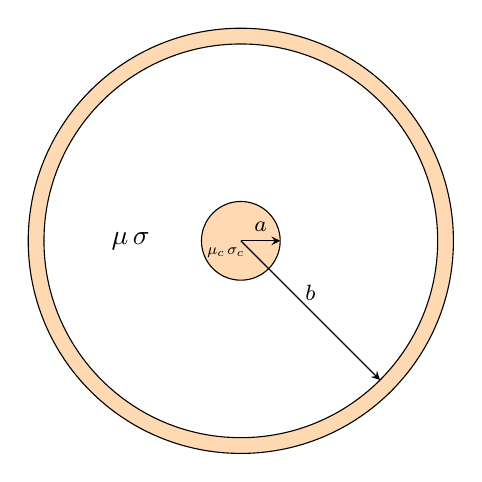
\begin{tikzpicture}
      \coordinate (O) at (0,0);
      \draw [fill=orange!30](O) circle (2.7);
      \draw  [fill=white](O) circle (2.5);
      \draw [fill=orange!30](O) circle (0.5);
      \draw[stealth-](0.5,0) -- (0,0)
      node[midway, above,font=\footnotesize] {$a$};
      \draw[stealth-](1.76775,-1.76775) -- (0,0)
      node[midway, above,font=\footnotesize] {$b$};
      \node (s) at (-1.4,0) {$\mu\,\sigma$};
      \node (s) [font=\footnotesize,scale=0.7] at (-0.19,-0.15) {$\mu_c\,\sigma_c$};
    \end{tikzpicture}  
  \end{center}\caption{Simplified coaxial section}
\end{figure}
The most common example of transmission line is the coaxial cable:\\
in our example we suppose the inner conductor radius $a$ and outer conductor radius $b$, then we also need to know the electric characteristic of the conductor ($\mu_c$ and $\sigma_c$) and the one of the separator ($\mu$ and $\sigma $). We can write now the characteristic value of the transmission line:
\begin{alignat*}{2}
    R&=\frac{R_s}{2\pi}\left(\frac{1}{a}+\frac{1}{b}\right)\;&&   \left[\si{\ohm\per\metre}\right]\\[5pt]
    L&=\frac{\mu}{2\pi}ln \left(\frac{b}{a}\right)&& \left[\si{\henry\per\metre}\right]\\[5pt]
    G&=\frac{2\pi\sigma}{ln\left(\frac{b}{a}\right)}&&\left[\si{\siemens\per\metre}\right]\\[5pt]
    C&=\frac{2\pi \epsilon}{ln\left(\frac{b}{a}\right)}&&\left[\si{\farad\per\metre}\right]
\end{alignat*}
$R_s$ is the resistance on the surface of the conductor and $R_s=\sqrt{\frac{\pi f \mu_c}{\sigma_c}}$.\\
Now let's make some consideration on $L$ and $C$:
\begin{equation}\label{eq:relation_LC_muepsilon}
  L\cdot C=\frac{\mu}{\cancel{2\pi}}\cancel{ln\left(\frac{b}{a}\right)}\frac{\cancel{2\pi}\,\varepsilon}{\cancel{ln\left(\frac{b}{a}\right)}}=\mu\cdot\varepsilon
\end{equation}
This relation $L\cdot C= \mu\cdot\varepsilon$ is very interesting for us, because we have already sen that $c=\frac{1}{\sqrt{\mu\,\varepsilon}}$ and $\beta=\omega\sqrt{\mu\,\varepsilon}$.\\
So what does the \cref{eq:relation_LC_muepsilon} mean? The answer is that when the EMF is forced to move inside a cable we will not use $\mu$ and $\varepsilon$, but $L$ and $C$, and that is very useful and cool for us.
\subsection*{Telegraph equations}
To obtain some cool relation for our TL we can use the Kirchhoff law as usual.
\begin{figure}[H]
  \begin{center}
      \begin{circuitikz} [ baseline=(current bounding box.center)]]
          \ctikzset { label/align = straight}
          \par\ctikzset{bipoles/resistor/width=.6,bipoles/resistor/height=.25}
          \draw (0,0)
          to[short, o-o,] (8,0)
          (0,4)to[short,i={$i(z,t)$},o-](1,4)
          to[R=$R\,\Delta z$] (2,4)
          to[L=$L\,\Delta z$] (4,4)
          to[short](7,4)
          to[short,i={$i(z+\Delta z,t)$},-o](8,4)
          (4,4)to[short](4,3)
          (3,3)to[short](5,3)
          (3,1)to[short](5,1)
          (4,0)to[short](4,1)
          (5,3)to[C=$C\,\Delta z$](5,1)
          (3,1)to[R=$G\,\Delta z$](3,3)
          (0,0)to[european voltages,open,v^={$v(z,t)$}](0,4)
          (8,0)to[european voltages,open,v_={$v(z+\Delta z,t)$}](8,4)
          (0,0) -- (8,0) node[midway,yshift=-1em]{$\Delta z$};
          ;
        \end{circuitikz}     
  \end{center} \caption{Circuital representation of a TL section with Kirchhoff}\label{eq:TL_with_kk}
\end{figure}
Now we can analyze the circuit in \cref{eq:TL_with_kk} using the Kirchhoff law:
\begin{equation*}
  v(z,t)-R\,\Delta z\,i(z,t)-L\,\Delta z\,\frac{\partial i(z,t)}{\partial t}=v(z+\Delta z,t)
\end{equation*}
Divide all for $\Delta z$
\begin{equation*}
  -\frac{v(z+\Delta z,t)-v(z,t)}{\Delta z}=R\,i(z,t)+L\,\frac{\partial i(z,t)}{\partial t}
\end{equation*}
Now let shrink the interval $\Delta z\rightarrow 0$
\begin{equation}\label{eq:Telegraph_eq}
  \begin{cases}
  -\frac{\partial v(z,t)}{\partial z}=R\,i(z,t)+L\frac{\partial i(z,t)}{\partial t}\\[5pt]
  -\frac{\partial i(z,t)}{\partial z}=G\,v(z,t)+C\frac{\partial v(z,t)}{\partial t}
  \end{cases}
\end{equation}
In \cref{eq:Telegraph_eq} we obtained the so called \emph{telegraph equations}.\\
The second equation in \cref{eq:Telegraph_eq} can be obtained by doing the same calculation that we have already done for the first one.\\
If we do not consider losses, those equations becomes even prettier:
\begin{equation}\label{eq:Telegraph_eq_prettier}
  \begin{cases}
  -\frac{\partial v(z,t)}{\partial z}=L\frac{\partial i(z,t)}{\partial t}\\[5pt]
  -\frac{\partial i(z,t)}{\partial z}=C\frac{\partial v(z,t)}{\partial t}
  \end{cases}
\end{equation}
\subsubsection*{Wave equation of the signal on the TL}
To obtain the wave equation, we can use the derivative over the space on the first equation of \cref{eq:Telegraph_eq_prettier}:
\begin{align}
  \begin{split}
  -\frac{\partial^2 v(z,t)}{\partial z^2}&=L\frac{\partial}{\partial t}\frac{\partial i(z,t)}{\partial z}\\[5pt]
  \frac{\partial^2 v(z,t)}{\partial z^2}&-L\,C\frac{\partial^2 v(z,t)}{\partial t^2}=0\\[5pt]
  \frac{\partial^2 v(z,t)}{\partial z^2}&-\frac{1}{c^2}\frac{\partial^2 v(z,t)}{\partial t^2}=0
  \end{split}\label{eq:wave_eq_on_TL}
\end{align}
The wave equation obtained in \cref{eq:wave_eq_on_TL} is very similar to what we have fond before, from here we can also obtain the solution of that equation:
\begin{equation}
  v(z,t)=V\bottomPlus \,\cos\left(\omega t-\frac{\omega}{c}z\right)+V\bottomMinus \,\cos\left(\omega t+\frac{\omega}{c}z\right)
\end{equation}
\subsubsection*{Telegraph and wave equation in phasor domain}
Starting from \cref{eq:Telegraph_eq_prettier} we can obtain the telegraph equation in phasor domain:
\begin{equation}
  \begin{cases}\label{eq:telegraph_in_phas_1}
  -\frac{\partial \phas{V}}{\partial z}=(R+j\omega L)\phas{I}\\[5pt]
  -\frac{\partial \phas{I}}{\partial z}=(G+j\omega C)\phas{V}
  \end{cases}
\end{equation}
Then the wave equation becomes:
\begin{align}
  \begin{split}
    &-\frac{\partial^2 \phas{V}}{\partial z^2}=(R+j\omega L)\frac{\partial \phas{I}}{\partial z}=\\[5pt]
    &=(R+j\omega L)(G+j\omega C)\phas{V}
  \end{split}
\end{align}
We introduce $\gamma = \sqrt{(R+j\omega L)(G+j\omega C)}=\alpha+j\beta$, then we obtain the telephone equation (another name for the wave equation for TL):
\begin{equation}
  \begin{cases}
  \frac{\partial^2 \phas{V}}{\partial z^2}-\gamma^2\,\phas{I}=0\\[5pt]
  \frac{\partial^2 \phas{I}}{\partial z^2}-\gamma^2\,\phas{V}=0
  \end{cases}\label{eq:telephone_eq}
\end{equation}
We can also write a beautiful solution from \cref{eq:telephone_eq}:
\begin{equation}\label{eq:voltage_in_phas_domain}
  \phas{V}(z)=V\bottomPlus \,e^{-\gamma z}+V\bottomMinus \,e^{\gamma z}
\end{equation}
We also know that $\gamma$ is a complex number, so what we can do is to write the same equation, but dividing $\gamma = \alpha+j\beta$ and looking only at the forward:
\begin{equation}
  \phas{V}(z)=V\bottomPlus \,e^{-\alpha z}\,e^{-j\beta z}
\end{equation}
If I go back to time domain (see \cref{eq:from_phas_to_time}):
\begin{equation}\label{eq:from_phas_to_time_TL}
  v(z,t)=V\bottomPlus e^{\alpha z}\cos(\omega t-\beta z)
\end{equation}
Inside $\gamma $ we have $R$,$L$,$G$ and $C$, so we have all the geometry and physical characteristic of the TL.
\subsubsection*{What could happen if we assume no losses?}
If we assume no losses over the line, then $\alpha=0$, and so $\gamma = j\beta$, then the wave propagation will follow \cref{eq:wave_solution_no_losses}:
\begin{equation}
  \begin{cases}
  \phas{V}(z)=V\bottomPlus \,e^{-j\beta z}+V\bottomMinus \,e^{j\beta z}=\phas{V_p}(z)+\phas{V_r}(z)\\[5pt]
  \phas{I}(z)=I\bottomPlus \,e^{-j\beta z}+I\bottomMinus \,e^{j\beta z}=\phas{I_p}(z)+\phas{I_r}(z)
  \end{cases}\label{eq:wave_solution_no_losses}
\end{equation}
So what are the parameters that give losses? We obtain the $\alpha$ and $\beta$ value from the real and imaginary value of:
\begin{align}
  \begin{split}
    \gamma &=\sqrt{(R+j\omega L)(G+j\omega C)}=\\[5pt]
    &=\sqrt{R\,G+j\omega L\,G+j\omega C\,R-\omega^2L\,C}=\\[5pt]
    &=\sqrt{j\omega( L\,G + C\,R)+R\,G-\omega^2L\,C}\\[5pt]
  \end{split}
\end{align}
I will not go further because I don't know how to do that, but the imaginary part is:
\begin{equation}
  \beta=\omega\sqrt{L\,C}
\end{equation}